La specifica delle politiche di sicurezza si basa su tre entità fondamentali:
\begin{itemize}
    \item \textbf{oggetti}: risorse che si vogliono proteggere (Es. tabelle)
    \item \textbf{soggetti}: chi può accedere agli oggetti specificati
    \item \textbf{privilegi}: quali operazioni può eseguire
\end{itemize}
Le autorizzazioni nel loro formato base possono essere rappresentate mediante una tupla $(s,o,p)$ dove:
\begin{itemize}
    \item $s$ \`e il soggetto
    \item $o$ \`e l'oggetto
    \item $p$ \`e il privilegio
\end{itemize}
Quando un utente vuole eseguire un operazione, il \textbf{gestore degli accessi} intercetta il comando e decide una delle seguenti autorizzazioni:
\begin{itemize}
    \item \textbf{totale}: l'accesso richiesto può essere totalmente eseguito
    \item \textbf{parziale}: sono una parte dell'accesso richiesto può essere eseguito
    \item \textbf{negata}: l'accesso richiesto non può essere eseguito
\end{itemize}

\subsection{SQL}
Esistono i comandi di \code{GRANT} e \code{REVOKE}:\vspace{2mm} \\
\code{GRANT \{<lista privilegi> | ALL PRIVILEGES\}\\
ON <nome oggetto>\\
TO \{<lista utenti> | <lista ruoli> | PUBLIC\}\\
\ [WITH GRANT OPTION]}
\vspace{2mm} \\
\code{REVOKE [GRANT OPTION FOR] <lista privilegi>\\
ON <nome oggetto>\\
FROM <lista utenti | <lista ruoli>>\\
\{RESTRICT | CASCADE\}}

\break
\subsection{Grafi}
Siccome le autorizzazioni possono essere date con \code{GRANT OPTION}, ogni operazione avrà associato un grafo rappresentante gli utenti e i loro permessi.

\begin{figure}[h]
    \centering
    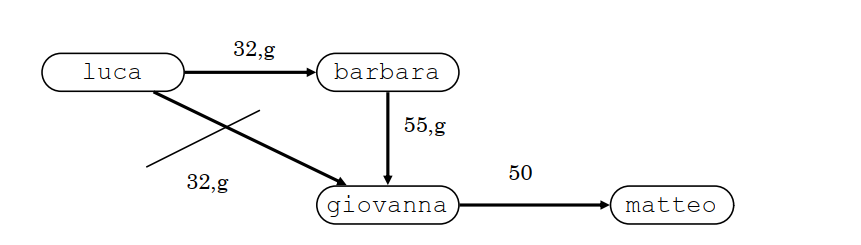
\includegraphics[width=0.8\textwidth, keepaspectratio]{grafoAccessi.png}
    \label{fig:grafo}
\end{figure}

\noindent Nell'esempio, abbiamo ogni nodo che rappresenta un utente, gli archi sono etichettati con $(\text{timestamp}, \text{grant\_option})$. Di solito, quando consideriamo un comando \code{REVOKE} non teniamo conto dei timestamp e quindi eliminando l'arco da Luca a Giovanna, l'arco con timestamp $50$ non viene eliminato anche se il timestamp sarebbe precedente a quello dell'unico arco rimanente.\\
In origine, il System R proponeva invece una soluzione che avrebbe tenuto conto. eliminando quindi l'arco da Giovanna a Matteo.

\subsection{Ruoli}
I ruoli sono una generalizzazione creata per assegnare a più utenti gli stessi privilegi.\\
Gli utenti possono ricoprire uno o più ruoli. Ogni utente che ricopre un ruolo acquisisce tutte le autorizzazioni ad esso connesse.\vspace{2mm} \\
\code{CREATE ROLE <nome ruolo>;}\\
\code{DROP ROLE <nome ruolo>;}\vspace{2mm} \\
L'utente può usare il seguente comando per cambiare ruolo (fra quelli a lui assegnati):\vspace{2mm} \\
\code{SET ROLE NomeRuolo}\vspace{2mm} \\
Per invece autorizzare un utente a ricoprire un ruolo si usa:\vspace{2mm} \\
\code{GRANT <lista ruoli concessi>\\
TO \{<lista utenti> | PUBLIC\}\\
\ [WITH ADMIN OPTION]}\vspace{2mm} \\
Per gestire le gerarchie si usa lo stesso comando sopra riportato elencando nel \code{TO} una lista di ruoli "padre".\vspace{2mm} \\
\code{GRANT commesso to direttoreVideoteca} $\Rightarrow$ direttoreVideoteca $\geq$ commesso